%-----------------------------------------------------------------------------------------------------------------------------------------------%
%	The MIT License (MIT)
%
%	Copyright (c) 2019 Jan Küster
%
%	Permission is hereby granted, free of charge, to any person obtaining a copy
%	of this software and associated documentation files (the "Software"), to deal
%	in the Software without restriction, including without limitation the rights
%	to use, copy, modify, merge, publish, distribute, sublicense, and/or sell
%	copies of the Software, and to permit persons to whom the Software is
%	furnished to do so, subject to the following conditions:
%	
%	THE SOFTWARE IS PROVIDED "AS IS", WITHOUT WARRANTY OF ANY KIND, EXPRESS OR
%	IMPLIED, INCLUDING BUT NOT LIMITED TO THE WARRANTIES OF MERCHANTABILITY,
%	FITNESS FOR A PARTICULAR PURPOSE AND NONINFRINGEMENT. IN NO EVENT SHALL THE
%	AUTHORS OR COPYRIGHT HOLDERS BE LIABLE FOR ANY CLAIM, DAMAGES OR OTHER
%	LIABILITY, WHETHER IN AN ACTION OF CONTRACT, TORT OR OTHERWISE, ARISING FROM,
%	OUT OF OR IN CONNECTION WITH THE SOFTWARE OR THE USE OR OTHER DEALINGS IN
%	THE SOFTWARE.
%	
%
%-----------------------------------------------------------------------------------------------------------------------------------------------%


%============================================================================%
%
%	DOCUMENT DEFINITION
%
%============================================================================%

%we use article class because we want to fully customize the page and don't use a cv template
\documentclass[10pt,A4]{article}	


%----------------------------------------------------------------------------------------
%	ENCODING
%----------------------------------------------------------------------------------------

% we use utf8 since we want to build from any machine
\usepackage[utf8]{inputenc}		

%----------------------------------------------------------------------------------------
%	LOGIC
%----------------------------------------------------------------------------------------

% provides \isempty test
\usepackage{xstring, xifthen}

%----------------------------------------------------------------------------------------
%	FONT BASICS
%----------------------------------------------------------------------------------------

% some tex-live fonts - choose your own

%\usepackage[defaultsans]{droidsans}
%\usepackage[default]{comfortaa}
%\usepackage{cmbright}
\usepackage[default]{raleway}
%\usepackage{fetamont}
%\usepackage[default]{gillius}
%\usepackage[light,math]{iwona}
%\usepackage[thin]{roboto} 

% set font default
\renewcommand*\familydefault{\sfdefault} 	
\usepackage[T1]{fontenc}

% more font size definitions
\usepackage{moresize}

%----------------------------------------------------------------------------------------
%	FONT AWESOME ICONS
%---------------------------------------------------------------------------------------- 

% include the fontawesome icon set
\usepackage{fontawesome}

% use to vertically center content
% credits to: http://tex.stackexchange.com/questions/7219/how-to-vertically-center-two-images-next-to-each-other
\newcommand{\vcenteredinclude}[1]{\begingroup
\setbox0=\hbox{\includegraphics{#1}}%
\parbox{\wd0}{\box0}\endgroup}

% use to vertically center content
% credits to: http://tex.stackexchange.com/questions/7219/how-to-vertically-center-two-images-next-to-each-other
\newcommand*{\vcenteredhbox}[1]{\begingroup
\setbox0=\hbox{#1}\parbox{\wd0}{\box0}\endgroup}

% icon shortcut
\newcommand{\icon}[3] { 							
	\makebox(#2, #2){\textcolor{maincol}{\csname fa#1\endcsname}}
}	

% icon with text shortcut
\newcommand{\icontext}[4]{ 						
	\vcenteredhbox{\icon{#1}{#2}{#3}}  \hspace{2pt}  \parbox{0.9\mpwidth}{\textcolor{#4}{#3}}
}

% icon with website url
\newcommand{\iconhref}[5]{ 						
    \vcenteredhbox{\icon{#1}{#2}{#5}}  \hspace{2pt} \href{#4}{\textcolor{#5}{#3}}
}

% icon with email link
\newcommand{\iconemail}[5]{ 						
    \vcenteredhbox{\icon{#1}{#2}{#5}}  \hspace{2pt} \href{mailto:#4}{\textcolor{#5}{#3}}
}

%----------------------------------------------------------------------------------------
%	PAGE LAYOUT  DEFINITIONS
%----------------------------------------------------------------------------------------

% page outer frames (debug-only)
% \usepackage{showframe}		

% we use paracol to display breakable two columns
\usepackage{paracol}

% define page styles using geometry
\usepackage[a4paper]{geometry}

% remove all possible margins
\geometry{top=1cm, bottom=1cm, left=1cm, right=1cm}

\usepackage{fancyhdr}
\pagestyle{empty}

% space between header and content
% \setlength{\headheight}{0pt}

% indentation is zero
\setlength{\parindent}{0mm}

%----------------------------------------------------------------------------------------
%	TABLE /ARRAY DEFINITIONS
%---------------------------------------------------------------------------------------- 

% extended aligning of tabular cells
\usepackage{array}

% custom column right-align with fixed width
% use like p{size} but via x{size}
\newcolumntype{x}[1]{%
>{\raggedleft\hspace{0pt}}p{#1}}%


%----------------------------------------------------------------------------------------
%	GRAPHICS DEFINITIONS
%---------------------------------------------------------------------------------------- 

%for header image
\usepackage{graphicx}

% use this for floating figures
% \usepackage{wrapfig}
% \usepackage{float}
% \floatstyle{boxed} 
% \restylefloat{figure}

%for drawing graphics		
\usepackage{tikz}				
\usetikzlibrary{shapes, backgrounds,mindmap, trees}

%----------------------------------------------------------------------------------------
%	Color DEFINITIONS
%---------------------------------------------------------------------------------------- 
\usepackage{transparent}
\usepackage{color}

% primary color
\definecolor{maincol}{RGB}{ 225, 0, 0 }

% accent color, secondary
% \definecolor{accentcol}{RGB}{ 250, 150, 10 }

% dark color
\definecolor{darkcol}{RGB}{ 70, 70, 70 }

% light color
\definecolor{lightcol}{RGB}{245,245,245}


% Package for links, must be the last package used
\usepackage[hidelinks]{hyperref}

% returns minipage width minus two times \fboxsep
% to keep padding included in width calculations
% can also be used for other boxes / environments
\newcommand{\mpwidth}{\linewidth-\fboxsep-\fboxsep}
	


%============================================================================%
%
%	CV COMMANDS
%
%============================================================================%

%----------------------------------------------------------------------------------------
%	 CV LIST
%----------------------------------------------------------------------------------------

% renders a standard latex list but abstracts away the environment definition (begin/end)
\newcommand{\cvlist}[1] {
	\begin{itemize}{#1}\end{itemize}
}

%----------------------------------------------------------------------------------------
%	 CV TEXT
%----------------------------------------------------------------------------------------

% base class to wrap any text based stuff here. Renders like a paragraph.
% Allows complex commands to be passed, too.
% param 1: *any
\newcommand{\cvtext}[1] {
	\begin{tabular*}{1\mpwidth}{p{0.98\mpwidth}}
		\parbox{1\mpwidth}{#1}
	\end{tabular*}
}

%----------------------------------------------------------------------------------------
%	CV SECTION
%----------------------------------------------------------------------------------------

% Renders a a CV section headline with a nice underline in main color.
% param 1: section title
\newcommand{\cvsection}[1] {
	\vspace{14pt}
	\cvtext{
		\textbf{\LARGE{\textcolor{darkcol}{\uppercase{#1}}}}\\[-4pt]
		\textcolor{maincol}{ \rule{0.1\textwidth}{2pt} } \\
	}
}

%----------------------------------------------------------------------------------------
%	META SKILL
%----------------------------------------------------------------------------------------

% Renders a progress-bar to indicate a certain skill in percent.
% param 1: name of the skill / tech / etc.
% param 2: level (for example in years)
% param 3: percent, values range from 0 to 1
\newcommand{\cvskill}[3] {
	\begin{tabular*}{1\mpwidth}{p{0.72\mpwidth}  r}
 		\textcolor{black}{\textbf{#1}} & \textcolor{maincol}{#2}\\
	\end{tabular*}%
	
	\hspace{4pt}
	\begin{tikzpicture}[scale=1,rounded corners=2pt,very thin]
		\fill [lightcol] (0,0) rectangle (1\mpwidth, 0.15);
		\fill [maincol] (0,0) rectangle (#3\mpwidth, 0.15);
  	\end{tikzpicture}%
}


%----------------------------------------------------------------------------------------
%	 CV EVENT
%----------------------------------------------------------------------------------------

% Renders a table and a paragraph (cvtext) wrapped in a parbox (to ensure minimum content
% is glued together when a pagebreak appears).
% Additional Information can be passed in text or list form (or other environments).
% the work you did
% param 1: time-frame i.e. Sep 14 - Jan 15 etc.
% param 2:	 event name (job position etc.)
% param 3: Customer, Employer, Industry
% param 4: Short description
% param 5: work done (optional)
% param 6: technologies include (optional)
% param 7: achievements (optional)
% param 8: URL (optional)

\newcommand{\cvevent}[8] {
	
	% we wrap this part in a parbox, so title and description are not separated on a pagebreak
	% if you need more control on page breaks, remove the parbox
	\parbox{\mpwidth}{
		\begin{tabular*}{1\mpwidth}{p{0.72\mpwidth}  r}
	 		\textcolor{black}{\textbf{#2}} & \colorbox{maincol}{\makebox[0.28\mpwidth]{\textcolor{white}{#1}}} \\
			\textcolor{maincol}{\textbf{#3}} & \\
			\ifthenelse{\isempty{#8}}{}{
			    \vspace{0.1pt}
                \small\iconhref {Globe} {12} {#8}{#8}{black}
    		}
		\end{tabular*}\\[8pt]
		
		\ifthenelse{\isempty{#4}}{}{
			\cvtext{#4}\\
		}
	}

	\ifthenelse{\isempty{#5}}{}{
		\vspace{9pt}
		{#5}
	}

	\ifthenelse{\isempty{#6}}{}{
		\vspace{9pt}
		\cvtext{\textbf{Technologies include:}}\\
		{#6}
	}

	\ifthenelse{\isempty{#7}}{}{
		\vspace{9pt}
		\cvtext{\textbf{Achievements include:}}\\
		{#7}
	}
	\vspace{14pt}
}

%----------------------------------------------------------------------------------------
%	 CV META EVENT
%----------------------------------------------------------------------------------------

% Renders a CV event on the sidebar
% param 1: title
% param 2: subtitle (optional)
% param 3: customer, employer, etc,. (optional)
% param 4: info text (optional)
\newcommand{\cvmetaevent}[4] {
	\textcolor{maincol} {\cvtext{\textbf{\begin{flushleft}#1\end{flushleft}}}}

	\ifthenelse{\isempty{#2}}{}{
	\textcolor{darkcol} {\cvtext{\textbf{#2}} }
	}

	\ifthenelse{\isempty{#3}}{}{
		\cvtext{{ \textcolor{darkcol} {#3} }}\\
	}

	\cvtext{#4}\\[14pt]
}

%---------------------------------------------------------------------------------------
%	QR CODE
%----------------------------------------------------------------------------------------

% Renders a qrcode image (centered, relative to the parentwidth)
% param 1: percent width, from 0 to 1
% param 2: qrcode file 
\newcommand{\cvqrcode}[2] {
	\begin{center}
		\includegraphics[width={#1}\mpwidth]{#2}
	\end{center}
}


%============================================================================%
%
%
%
%	DOCUMENT CONTENT
%
%
%
%============================================================================%
\begin{document}
\columnratio{0.31}
\setlength{\columnsep}{2.2em}
\setlength{\columnseprule}{4pt}
\colseprulecolor{lightcol}
\begin{paracol}{2}
\begin{leftcolumn}
%---------------------------------------------------------------------------------------
%	META IMAGE
%----------------------------------------------------------------------------------------
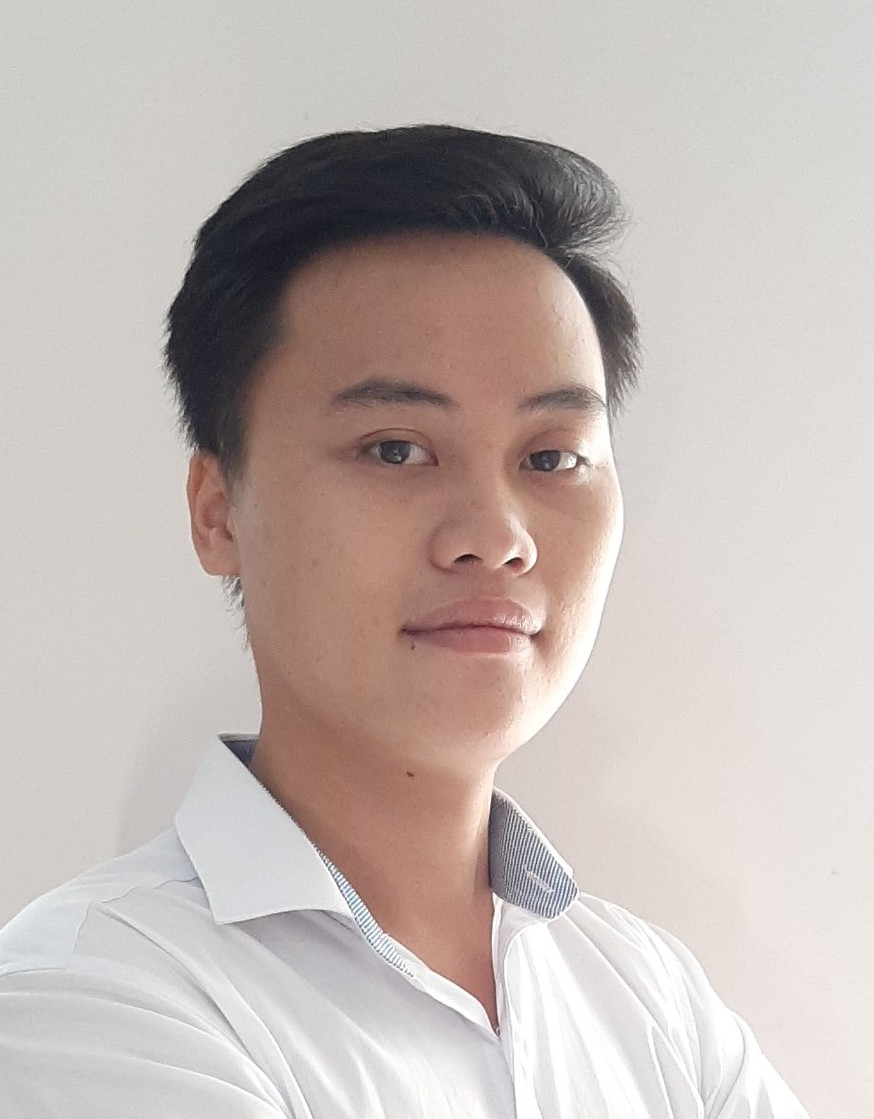
\includegraphics[width=\linewidth]{avatar.jpg}	%trimming relative to image size

%---------------------------------------------------------------------------------------
%	META SKILLS
%----------------------------------------------------------------------------------------
\cvsection{SKILLS}

\cvskill{JavaScript} {5+ yrs} {1} \\[-2pt]

\cvskill{ReactJS} {4+ yrs} {0.95} \\[-2pt]

\cvskill{React Native} {3+ yrs} {0.8} \\[-2pt]

\cvskill{NodeJS/Java} {2+ yrs} {0.6} \\[-2pt]

\cvskill{VueJS/Flutter} {2+ yrs} {0.4} \\[-2pt]

\cvskill{GIT} {4+ yrs} {0.75} \\[-2pt]

\cvskill{Linux/Unix} {3+ yrs} {0.5} \\[-2pt]

\cvskill{Open Source Tools} {} {0.4} \\[-2pt]



\vfill\null
\cvsection{CONTACT}

\icontext{MapMarker}{12}{126 Nguyen Cu Trinh\\District 1, HCMC}{black}\\[6pt]
\icontext{MobilePhone}{12}{+84 335 114 115}{black}\\[6pt]
\iconemail{Envelope}{12}{daoquocvuong@gmail.com}{daoquocvuong@gmail.com}{black}\\[6pt]
\iconhref {Github} {12} {git/blackwine93v}{https://github.com/blackwine93v}{black}\\[6pt]
\iconhref {Linkedin} {12} {linkedin/blackwine93v}{https://www.linkedin.com/in/blackwine93v/}{black}\\[6pt]
\cvqrcode{0.4}{git-qrcode}


%---------------------------------------------------------------------------------------
%	TALKS
%----------------------------------------------------------------------------------------
\newpage
\cvsection{TALKS}
\cvmetaevent
{Nov 2017}
{ReactJS 101 Workshop}
{SPEAKER AT NEIGHBORHUB CO-WORKING SPACE}
{
    \cvlist {
        \item Introduced the ReactJS - A modern web application development.
        \item How does ReactJS work?
        \item How to build a ReactJS application?
    }
}

\cvmetaevent
{Dec 2017}
{Internal Company Training}
{PRESENTER FOR SUNRISE SOFTWARE SOLUTION’S EMPLOYEES}
{
    \cvlist {
        \item Introduced the ReactJS - ReactJS concepts.
        \item Shared common use cases, best practices when using ReactJS.
        \item Built a ReactJS application with ReduxJS, ImmutableJS.
    }
}

%---------------------------------------------------------------------------------------
%	EDUCATION
%----------------------------------------------------------------------------------------
\newpage
\cvsection{EDUCATION}

\cvmetaevent
{2011 - 2015}
{B.S. IN COMPUTER NETWORKING}
{University Of Science, HCMC}
{
    \cvlist {
        \item Annual College Scholarship.
        \item GPA: 8.21
    }
}


% \newpage
% \mbox{} % hotfix to place qrcode on the bottom when there are not other elements
% \vfill
% \cvqrcode{0.7}{qrcode}

\end{leftcolumn}
\begin{rightcolumn}
%---------------------------------------------------------------------------------------
%	TITLE  HEADER
%----------------------------------------------------------------------------------------
\fcolorbox{white}{darkcol}{\begin{minipage}[c][3.5cm][c]{1\mpwidth}
	\begin {center}
		\HUGE{ \textbf{ \textcolor{white}{ \uppercase{ VUONG DAO } } } } \\[-24pt]
		\textcolor{white}{ \rule{0.1\textwidth}{1.25pt} } \\[4pt]
		\large{ \textcolor{white} {Software Engineer} }
	\end {center}
\end{minipage}} \\[14pt]
\centering{
    \small\textcolor{black} {
        \textit{ "You cannot solve a problem with the same mind that created it" } \\
        - ALBERT EINSTEIN -
    }\\[4pt]
}
\vspace{-12pt}

%---------------------------------------------------------------------------------------
%	PROFILE
%----------------------------------------------------------------------------------------
\vfill\null
\cvsection{PROFILE}

\cvtext{Software Engineer, specialized in frontend as web and mobile development, experienced with medium and large projects, strong JavaScript, and a passion for OpenSource software.\\

Highly motivated to work in a team, both comfortable in big companies as in small teams.\\

Pursue the path to become a Solution Architect.
}
\vfill\null

%---------------------------------------------------------------------------------------
%	WORK EXPERIENCE
%----------------------------------------------------------------------------------------
\vfill\null
\cvsection{WORK EXPERIENCE}

\cvevent
	{10/2019 - 04/2020}
	{Software Engineer}
	{INCOGNITO - Privacy Mode for Cryptocurrency}
	{Building websites, wallet mobile app, IncognitoJS SDK to interact with the Incognito chain.}
	{\cvlist{
	    \item Designed application architect and built wallet app (Incognito: Privacy-Preserving Crypto Wallet).
		\item Built landing pages for launching Incognito nodes, Incognito wallet.
		\item Maintained wallet chrome extension and wallet web.
		\item Released open-source IncognitoJS SDK and documentations.
		\item Released open-source IncognitoJS React Native package.
		\item Researched a solution to improve the time of creating a privacy transaction from 10 minutes to 30 seconds.
		\item Optimized application performance and checked for security vulnerabilities.
	}}
	{\cvlist {
		\item ReactJS, ReduxJS, Pug, SCSS, LESS, Web component.
		\item React Native, Gomobile, Webassembly.
		\item Service worker for building PWA.
		\item Lazing loading, code splitting.
		\item GIT, yarn, Webpack, Linux tools.
	}}
	{}
	{https://github.com/incognitochain}
	
\newpage
\vfill\null
\cvevent
	{04/2018 - 04/2020}
	{Software Engineer}
	{MECHANICDESK - Workshop Management Software}
	{Building websites, mobile app for managing and tracking jobs, cars, invoices, etc. of a mechanic workshop.}
	{\cvlist{
	    \item Designed application architect and built MechanicDesk app.
		\item Built Support Portal website for admins.
	    \item Built Dealer Ship website to manage cars.
	}}
	{\cvlist {
		\item Flutter (Dart), Dart Redux.
		\item VueJS, Pug, SCSS.
		\item Unit testing with Mocha, Jest, Sinon.
		\item Test-driven development, code coverage.
		\item Lazing loading, code splitting.
		\item GIT, yarn, Webpack, Linux tools.
	}}
	{}
	{https://www.mechanicdesk.com.au}


\vfill\null
\cvevent
	{09/2018 - 09/2019}
	{Frontend Engineer}
	{CONSTANT - P2P Lending}
	{Responsible for initializing and developing a high traffic secure peer-to-peer lending platform website that using ReactJS.}
	{\cvlist{
	    \item Designed application architect.
		\item Implemented features.
		\item Built Progressive Web App (PWA).
		\item Optimized application performance and checked for security vulnerabilities.
	}}
	{\cvlist {
		\item ReactJS, Bootstrap, ReduxJS.
		\item ExpressJS for server-side rendering.
		\item Service worker for building PWA.
		\item Lazing loading, code splitting.
		\item GIT, yarn, Webpack.
	}}
	{}
	{https://www.myconstant.com}

\newpage
\vfill\null
\cvevent
	{04/2018 - 08/2018}
	{Frontend Engineer}
	{EYEVIEW - INSIGHTUS}
	{Built a web application allows tracking public cameras of the Australia government.\\
	Support managing, monitoring, viewing and making live stream on these cameras.}
	{\cvlist{
	    \item Integrated 2D/3D geographical maps/objects.
		\item Implemented tracking drones locations.
		\item Built managing view for CCTVs (cameras).
		\item Optimized application performance.
	}}
	{\cvlist {
		\item AngularJS, Bootstrap, SCSS.
		\item CesiumJS (3D map), Leaflet (2D map).
		\item HLS live streaming video.
		\item Docker.
		\item GIT, npm, Webpack.
	}}
	{}
	{https://insightus.com.au/Eyeview}

\vfill\null
\cvevent
	{11/2017 - 03/2018}
	{Frontend Engineer}
	{THX STANDARD}
	{THX Standard website offers test scores and comparisons of A/V products, using Angular for intuitive frontend.}
	{\cvlist{
	    \item Designed application architect.
		\item Implemented features.
		\item Optimized application performance: loading speed, SEO.
		\item Responsive for mobile-friendly.
	}}
	{\cvlist {
		\item AngularJS, Bootstrap, SCSS.
		\item Restful API.
		\item Docker.
		\item GIT, npm, Webpack.
	}}
	{}
	{https://www.thxstandard.com}

\vfill\null
\newpage
\cvevent
	{04/2017 - 10/2017}
	{Mobile Engineer}
	{TRIPPER. MATKA- JA KULULASKUT}
	{Responsible for building a mobile application both Android and iOS, \\
	support automatically makes a travel invoice with a calendar entry and adds all receipts to customer books without writing a word.}
	{\cvlist{
		\item Implemented and enhanced new features.
		\item Optimized application performance and reducing the size.
		\item Maintenance.
	}}
	{\cvlist {
		\item React Native.
		\item ImmutableJS, Redux, Firebase.
		\item Text Recognition.
		\item GIT, Yarn.
	}}
	{}
	{https://gettripper.com}
	
\vfill\null
\cvevent
	{01/2016 - 03/2017}
	{FullStack Engineer}
	{Taembe.vn}
	{Built and maintained an e-commerce website that using ReactJS and Hapi server.}
	{\cvlist{
		\item Designed and implemented UI/UX.
		\item Implemented Restful API in Node.js Hapi.
		\item Integrated SendGrid, Mixpanel, Social authentication, and online payment Stripe.
		\item Built mobile app.
	}}
	{\cvlist {
		\item Frontend: ReactJs, Bootstrap3.
		\item Backend: HapiJS, Magento, CouchDB.
		\item Mobile app: Java.
		\item Server-side rendering, lazy loading, bundle splitting.
		\item Gulp, GIT, npm, AWS.
	}}
	{}
	{}

% hotfixes to create fake-space to ensure the whole height is used
\mbox{}
\vfill
\mbox{}
\vfill
\mbox{}
\vfill
\mbox{}
\end{rightcolumn}
\end{paracol}
\end{document}

